\documentclass[10 pt,usenames,dvipsnames, oneside]{article}
\usepackage{../../../modelo-ensino-medio}


\begin{document}

\begin{center}
  \begin{minipage}[l]{3cm}
\includegraphics[width=2cm]{logo}    
\end{minipage}\hfill
\begin{minipage}[r]{.8\textwidth}
 {\Large \scshape Atividade: A água está subindo}  
\end{minipage}
\end{center}
\vspace{.2cm}

\ifdefined\prof
\begin{objetivos}
\item \textbf{LAF2} Compreender a taxa de variação como uma medida de covariação entre grandezas e utilizá-la para interpretar situações reais.
\end{objetivos}

\begin{goals}
\begin{enumerate}

\item [OE1] Associar uma situação real a uma representação gráfica.

\item [OE2] Diferenciar situações de crescimento, identificando quando o gráfico pode ser uma linha reta – taxa de variação constante (parte I) e quando não (parte II).

\item [OE3] Diferenciar entre situações em que há taxa de variação constante (parte III).

\end{enumerate}

\tcblower

\begin{itemize}
\item Considere realizar essa atividade em grupo, principalmente em turmas maiores. Essa pode ser uma estratégia interessante para dar oportunidade para que os estudantes, em grupos, exponham suas impressões e argumentos.

\item Na parte I espera-se que os estudantes descartem rapidamente o gráfico decrescente. Certifique-se de que as justificativas contenham elementos suficientes que permitam diferenciar entre os dois gráficos crescentes.
\item Podem aparecer respostas imprecisas do tipo: "o recipiente tem os lados retos". Peça aos estudantes que sejam o mais específicos possível.
\item Não faz parte dos objetivos dessa atividade que os estudantes encontrem as fórmulas que fornecem as alturas em função do tempo.
\item Na parte III, conduza os estudantes a perceber que há uma relação decrescente entre o raio do cilindro e a taxa de variação (quanto menor o raio, maior a inclinação da reta). De fato, a taxa de variação é inversamente proporcional ao quadrado do raio.
\end{itemize}

\end{goals}

\bigskip
\begin{center}
{\large \scshape Atividade}
\end{center}
\fi

\textbf{Parte I} Um reservatório cilíndrico de altura $h$ (em cm), com capacidade máxima de $100 \ell$ encontra-se vazio. Para enchê-lo, abriu-se uma torneira que despeja $2\ell$ de água por minuto.

\begin{figure}[H]
\centering
\includegraphics[width=100bp]{taxa-ativ-1-1}

%\caption{}
\label{}
\end{figure}

Qual dos gráficos seguintes expressa corretamente a variação da altura $x$ da coluna de água em função do tempo $t$? Explique.

\setlength{\columnsep}{0pt}
\begin{multicols}{3}
\begin{enumerate}[label=(\Roman*)]
\item
\adjustbox{valign=t}{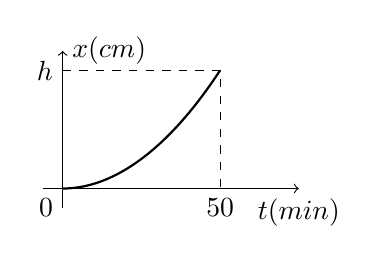
\begin{tikzpicture}[scale=.5,baseline=(current bounding box.north)]

\draw [->] (-.5,0) -- (6,0) node [below ] {$t(min)$};
\draw [->] (0,-.5) -- (0,3.5) node [right] {$x(cm)$};
\draw [dashed] (0,3) -- (4,3) -- (4,0);
\node [left] at (0,3) {$h$};
\node [below left] at (0,0) {$0$};
\node [below] at (4,0) {$50$};

\draw [thick] (0,0) parabola (4,3);
\end{tikzpicture}}

\item
\adjustbox{valign=t}{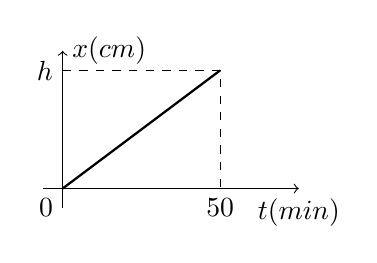
\begin{tikzpicture}[scale=.5,baseline=(current bounding box.north)]

\draw [->] (-.5,0) -- (6,0) node [below ] {$t(min)$};
\draw [->] (0,-.5) -- (0,3.5) node [right] {$x(cm)$};
\draw [dashed] (0,3) -- (4,3) -- (4,0);
\node [left] at (0,3) {$h$};
\node [below left] at (0,0) {$0$};
\node [below] at (4,0) {$50$};

\draw [thick] (0,0) -- (4,3);
\end{tikzpicture}}


\item
\adjustbox{valign=t}{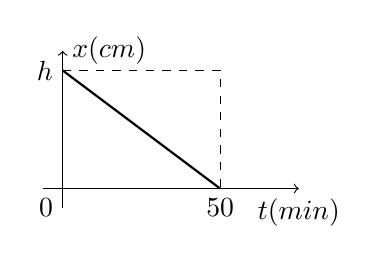
\begin{tikzpicture}[scale=.5,baseline=(current bounding box.north)]

\draw [->] (-.5,0) -- (6,0) node [below ] {$t(min)$};
\draw [->] (0,-.5) -- (0,3.5) node [right] {$x(cm)$};
\draw [dashed] (0,3) -- (4,3) -- (4,0);
\node [left] at (0,3) {$h$};
\node [below left] at (0,0) {$0$};
\node [below] at (4,0) {$50$};

\draw [thick] (0,3) -- (4,0);
\end{tikzpicture}}
\end{enumerate}
\end{multicols}

\textbf{Parte II} Um reservatório cônico de altura $h$ (em cm), com capacidade máxima de $100\ell$, encontra-se vazio e posicionado com o vértice para baixo, conforme mostra a figura. Para enchê-lo, abriu-se uma torneira que despeja $2\ell$ de água por minuto.

\begin{figure}[H]
\centering
\includegraphics[width=100bp]{taxa-ativ-1-3}

%\caption{}
\label{}
\end{figure}

Qual dos gráficos seguintes expressa corretamente a variação da altura $x$ da coluna de água em função do tempo $t$? Explique.

\setlength{\columnsep}{0pt}
\begin{multicols}{3}
\begin{enumerate}[label=(\Roman*)]
\item \adjustbox{valign=t}{
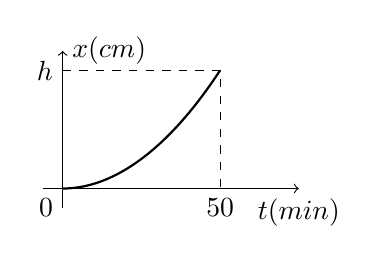
\begin{tikzpicture}[scale=.5,baseline=(current bounding box.north)]

\draw [->] (-.5,0) -- (6,0) node [below ] {$t(min)$};
\draw [->] (0,-.5) -- (0,3.5) node [right] {$x(cm)$};
\draw [dashed] (0,3) -- (4,3) -- (4,0);
\node [left] at (0,3) {$h$};
\node [below left] at (0,0) {$0$};
\node [below] at (4,0) {$50$};

\draw [thick] (0,0) parabola (4,3);
\end{tikzpicture}}

\item
\adjustbox{valign=t}{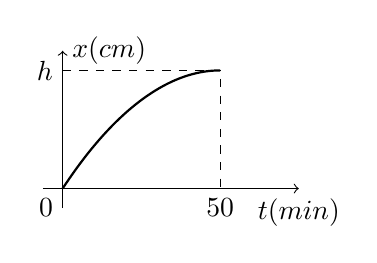
\begin{tikzpicture}[scale=.5,baseline=(current bounding box.north)]

\draw [->] (-.5,0) -- (6,0) node [below ] {$t(min)$};
\draw [->] (0,-.5) -- (0,3.5) node [right] {$x(cm)$};
\draw [dashed] (0,3) -- (4,3) -- (4,0);
\node [left] at (0,3) {$h$};
\node [below left] at (0,0) {$0$};
\node [below] at (4,0) {$50$};

\draw [thick] (4,3) parabola (0,0);
\end{tikzpicture}}


\item
\adjustbox{valign=t}{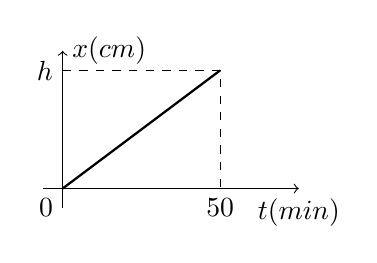
\begin{tikzpicture}[scale=.5,baseline=(current bounding box.north)]

\draw [->] (-.5,0) -- (6,0) node [below ] {$t(min)$};
\draw [->] (0,-.5) -- (0,3.5) node [right] {$x(cm)$};
\draw [dashed] (0,3) -- (4,3) -- (4,0);
\node [left] at (0,3) {$h$};
\node [below left] at (0,0) {$0$};
\node [below] at (4,0) {$50$};

\draw [thick] (0,0) -- (4,3);
\end{tikzpicture}}
\end{enumerate}
\end{multicols}

\textbf{PARTE III} Os recipientes cilíndricos $A,B, \text{ e } C$, que têm altura $h$ raios da base respectivamente iguais a $r,2r$ e $3r$, estão vazios. As torneiras que os abastecem estão igualmente reguladas para despejar o mesmo número de litros de água por minuto.

\begin{figure}[H]
\centering
\includegraphics[width=150bp]{taxa-ativ-1-5}

%\caption{}
\label{}
\end{figure}

Os gráficos mostram a varação da altura $x$ da coluna de água em função to tempo $t$. Associe cada recipiente ao gráfico correspondente a ele e justifique suas escolhas.

\begin{enumerate}[label=(\Roman*)]
\begin{multicols}{3}
\centering

\item\adjustbox{valign=t}{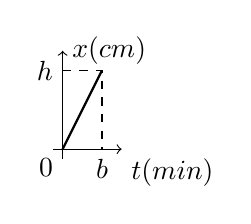
\begin{tikzpicture}[scale=.25,baseline=(current bounding box.north)]

\draw [->] (-.5,0) -- (3,0) node [below right] {$t(min)$};
\draw [->] (0,-.5) -- (0,5) node [right] {$x(cm)$};
\draw [dashed] (0,4) -- (2,4) -- (2,0);
\node [left] at (0,4) {$h$};
\node [below left] at (0,0) {$0$};
\node [below] at (2,0) {$b$};

\draw [thick] (0,0) -- (2,4);
\end{tikzpicture}}


\item\adjustbox{valign=t}{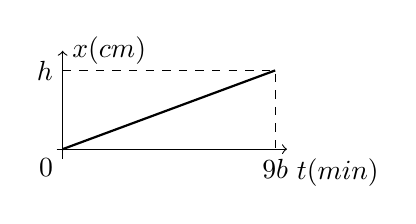
\begin{tikzpicture}[scale=.25,baseline=(current bounding box.north), xscale=.6]

\draw [->] (-.5,0) -- (19,0) node [below right] {$t(min)$};
\draw [->] (0,-.5) -- (0,5) node [right] {$x(cm)$};
\draw [dashed] (0,4) -- (18,4) -- (18,0);
\node [left] at (0,4) {$h$};
\node [below left] at (0,0) {$0$};
\node [below] at (18,0) {$9b$};

\draw [thick] (0,0) -- (18,4);
\end{tikzpicture}}

\item\adjustbox{valign=t}{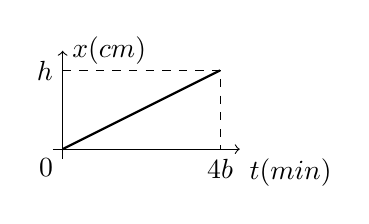
\begin{tikzpicture}[scale=.25,baseline=(current bounding box.north), ]

\draw [->] (-.5,0) -- (9,0) node [below right] {$t(min)$};
\draw [->] (0,-.5) -- (0,5) node [right] {$x(cm)$};
\draw [dashed] (0,4) -- (8,4) -- (8,0);
\node [left] at (0,4) {$h$};
\node [below left] at (0,0) {$0$};
\node [below] at (8,0) {$4b$};

\draw [thick] (0,0) -- (8,4);
\end{tikzpicture}}

\end{multicols}
\end{enumerate}

\ifdefined\prof

\begin{solucao}

\textbf{(Parte I)}: Gráfico (II). O reservatório tem a forma de um cilíndro e a água entre a uma vazão constante.

\textbf{(Parte II)}: Gráfico (II). Devido a forma de cone do reservatório, inicialmente a coluna de água sobe mais rapidamente. Posteriormente, como a vazão de entrada de água no recipiente permanece constante durante todo o tempo, a altura da coluna sobe mais lentamente.

\textbf{(Parte III)}: A coluna de água subirá mais rapidamente no reservatório mais estreito e mais lentamente no reservatório mais largo. Dessa forma, o reservatório A está associado ao gráfico (I), o B ao gráfico (III) e o C ao gráfico (II).
\end{solucao}
\fi

\end{document}